\section{منظم‌سازی}

برای جلوگیری از بیش‌برازش مدل‌ها می‌توانیم از منظم‌سازی\LTRfootnote{Regularization} استفاده کنیم. امکان‌ دارد گاهی با شرایطی مواجه شویم که ۲ یا چند تابع قادر به کاهش خطای مورد نظر بر روی داده‌های آموزش شوند. حال پرسشی که مطرح می‌شود این است که کدام یک از این توابع عملکرد بهتری بر روی داده‌های آزمون خواهد داشت؟

برای پاسخ به این پرسش به یک اصل فلسفی به نام تیغ اوکام\LTRfootnote{Occam's razor (Ockham's razor)} رجوع می‌کنیم. این اصل به زبان ساده بیان می‌کند که «میان دو نگره‌ که توان توصیف و پیش‌بینی یکسانی دارند، ساده‌ترین را برگزین» و در اینجا با اتکا بر این اصل، تلاش می‌کنیم که در انتخاب توابع و مدل‌ها، ساده‌ترین را ترجیح دهیم.

% با استفاده از نظریه یادگیری آماری می‌توانیم ظرفیت مدل‌ها را به صورت کمی مقایسه کنیم تا روشی برای تشخیص سادگی مدل‌های مختلف داشته باشیم. یکی از روش‌های متدوال برای انجام این کار، بررسی بُعد $\text{\begin{latin}VC\end{latin}}$\LTRfootnote{Vapnik-Chervonekis dimension} است که ظرفیت یک دسته‌بند دوتایی\LTRfootnote{binary classifier} را اندازه‌گیری می‌کند.

اگر بتوانیم میزان پیچیدگی و سادگی مدل‌های مختلف را به صورت کمی مقایسه کنیم، با افزودن ضریبی از آن مقدار کمی به تابع هزینه اولیه می‌توانیم ترجیح توابع ساده‌تر را به زبان ریاضی بیان کنیم. برای نمونه اگر تابع هزینه $J(w)$ را داشته باشیم، می‌توانیم آن را به صورت زیر تغییر دهیم:
$$J_\lambda(w) = J(w) + \lambda R(w)$$
که در اینجا $\lambda$ یک ابرپارامتر\LTRfootnote{hyperparameter} است و $R(w)$ یک تابع منظم‌سازی است که در روش‌های کلاسیک اغلب تابعی از پارامتر‌های مدل می‌باشد. اگر مقادیر زیاد $R(w)$ متناظر با پیچیدگی بیشتر و مقادیر کم متناظر با سادگی باشند، تابع هزینه جدید از میان مدل‌هایی که $J(w)$ تقریباً برابر دارند، مدلی که ساده‌تر است را به عنوان پاسخ بهینه معرفی می‌کند. مقدار $\lambda$ تعیین می‌کند که تا چه اندازه سادگی مدل برای ما اهمیت دارد. اگر این مقدار برابر با صفر باشد هیچ محدودیتی بر روی پیچیدگی مدل اعمال نمی‌شود و در صورتی که مقدار آن را افزایش دهیم،‌اهمیت بیشتری به سادگی مدل داده خواهد شد.

\begin{figure}
    \centering
    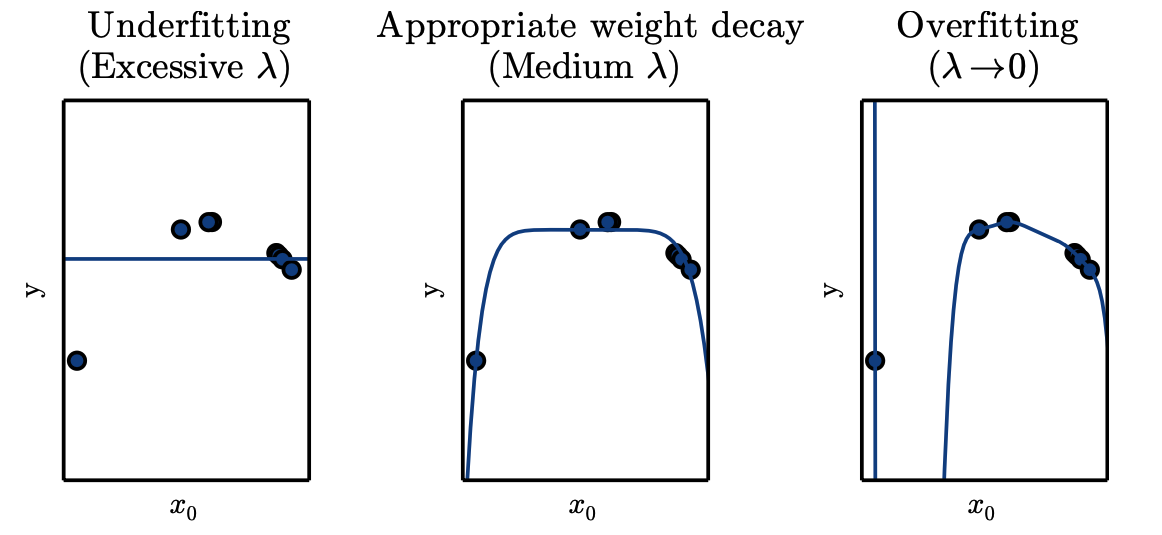
\includegraphics[width=\textwidth]{figs/Regularization.png}
    \caption{ مسئله‌‌ای که در شکل \ref{fig:Capacity} بررسی کردیم را به یاد بیاورید. در اگر ندانیم تابع واقعی از درجه ۲ است، مجبور می‌شویم که برای یافتن ظرفیت مناسب درجات مختلف را بررسی کنیم. هنگامی که مسائل پیجیده‌تر مواجه شویم این امر امکان‌پذیر نخواهد بود و یافتن ظرفیت ایده‌آل بسیار وقت‌گیر و یا حتی غیرممکن خواهد شد. یک راه برای جلوگیری از این مشکل این است که مدلی با ظرفیت بالا را انتخاب کرده و با منظم‌سازی تلاش کنیم تا به پاسخی قابل‌قبول برسیم که عملکرد تقریباً مشابهی نسبت به حالت ایده‌آل داشته باشد. در اینجا یک چندجمله‌ای درجه ۹ را با مقادیر مختلف $\lambda$ آموزش دادیم. (راست) در صورتی که مقدار $\lambda$ برابر با صفر باشد عملاً هیچ منظم‌سازی رخ نداده و همچنان بیش‌برازش رخ می‌دهد. (چپ) در صورتی که مقدار $\lambda$ بیش از اندازه زیاد باشد هیچ یادگیری صورت نگرفته و کم‌برازش رخ می‌دهد. (وسط) در صورتی که مقدار معقولی برای $\lambda$ انتخاب شود، مدل نهایی برخلاف ظرفیت بالاتری که نسبت به ظرفیت واقعی دارد، عملکرد مناسبی خواهد داشت.}
    \label{fig:Regularization}
\end{figure}

برای منظم‌سازی روش‌های متعددی وجود دارد. یک روش متداول برای انجام این کار روش کاهش وزن‌ها\LTRfootnote{weight decay} است که در رگرسیون خطی، یادگیری ژرف\LTRfootnote{deep learning} و ... استفاده می‌شود. با نظر گرفتن نرم‌های $\ell_2$ وزن‌ها به عنوان تابع منظم‌سازی می‌باشد. با انجام این کار وزن‌های کوچک‌تر نسبت به وزن‌های بزرگ‌تر ترجیح داده می‌شوند. در این صورت وزرن‌های بزرگ‌تر تنها در صورتی انتخاب می‌شوند که بتوانند مقدار خطای آموزش را به طرز چشمگیری در مقایسه با وزن‌های کوچک‌تر کاهش دهند. اگر بجای نرم $\ell_2$ از نرم $\ell_1$ استفاده کنیم، وزن‌های تنک\LTRfootnote{sparse} ترجیح داده می‌شوند.
در شکل \ref{fig:Regularization} می‌توانید اثرات این نوع منظم‌سازی که از نرم $\ell_2$ استفاده می‌کند را ببینید. 

از دیگر روش‌های منظم‌سازی می‌توان به توقف زودهنگام\LTRfootnote{early stopping} اشاره کرد. بسیاری از الگوریتم‌های یادگیری ماشین به صورت مرحله به مرحله بهبود می‌یابند. در این موارد اغلب با بروزرسانی پارامتر‌ها تلاش می‌کنیم تا خطای آموزش را به صورت پی در پی کاهش دهیم تا به پارامتر‌ها و یا وزن‌های بهینه برسیم. اما امکان دارد که پارامتر‌هایی که متناظر با خطای کمینه باشند، با حفظ خواص مجموعه داده‌های آموزش به این دستاورد برسند و نتوانند به خوبی بر روی داده‌های آزمون تعمیم یابند. یک روش برای پیشگیری از بروز چنین مشکلاتی توقف زودهنگام الگوریتم است. در این صورت شرایط توقف زودهنگام (تعداد مراحل، خطای توقف، ...) را می‌توان به صورت یک ابرپارامتر در نظر گرفت. این روش از منظم‌سازی در آموزش‌ درخت‌های تصمیم\LTRfootnote{decision tree}، جنگل‌های تصادفی\LTRfootnote{random forest}، شبکه‌های عصبی\LTRfootnote{neural network} و ... استفاده می‌شود.

اکنون امکان دارد که این پرسش مطرح شود که چگونه می‌توانیم ابرپارامتر‌های مناسب برای آموزش مدل‌هایمان را پیدا کنیم؟ در بخش بعدی نگاهی به روش‌هایی برای یافتن ابرپارامتر‌های بهینه و مفهوم صحت‌سنجی\LTRfootnote{validation} می‌اندازیم.